\documentclass[11pt,t]{beamer}
\usetheme[kulak]{kuleuven2}	%THEME OPTIONS for LOGO: kul (default), kulak, lrd,    ; OPTIONS for TITLE PAGE: normal (default), sedes


%%% OTHER SETTINGS
\usefonttheme[onlymath]{serif}			% math font with serifs, delete to make it sans-serif
\setbeamertemplate{footline}[body] 		% delete this line to remove footline bar on all frames
\usepackage[orientation=landscape,size=custom,width=16,height=9,scale=0.5,debug]{beamerposter}


%%% ADDED PACKAGES:
\usepackage[english]{babel}
\usepackage{amsfonts}
\usepackage{amssymb}


%%% TITLE PAGE INFO:
\title[Footer]{Algorithms and Data Structures} %[]] will appear in footline
\subtitle{Chapter 18: B-Trees\\(based on book “Introduction to Algorithms” of Cormen et al.)}

\author{Vincent Van Schependom}
\institute{KU Leuven Campus Kulak Kortrijk}
\date{Academiejaar 2024--2025}




\begin{document}
	\csname beamer@calculateheadfoot\endcsname %recalculate head and foot dimension


	%%
	%%  0. TITLE PAGE and TABLE OF CONTENT
	%%
	% Title page
	\begin{frame}[plain,noframenumbering]
		\titlepage
	\end{frame}


	% Table of Contents
	\begin{frame}{Outline}
		\hfill	{\large \parbox{.961\textwidth}{\tableofcontents[hideothersubsections]}}
	\end{frame}



	\section{Introduction}

	\begin{frame}{Double--column frame}
		\begin{columns}
			\begin{column}{.5\textwidth}
				\centering
				\begin{figure}
					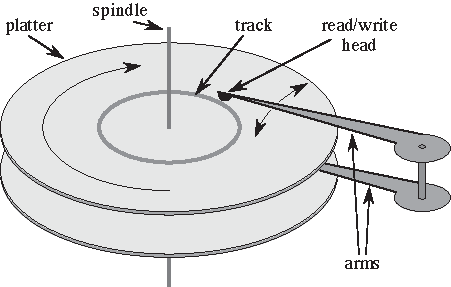
\includegraphics[width=\columnwidth]{images/disk}
				\end{figure}
			\end{column}
			\begin{column}{.5\textwidth}
				This is the top of the second column.
			\end{column}
		\end{columns}
	\end{frame}


	%%
	%%  SECTION 1 - INFO
	%%
	\section{Definition of a B-Tree}

	\begin{frame}[noframenumbering]{Definition of a B-Tree}
		\begin{itemize}[<+->]
			\item Rooted tree with root \(T.root\)
			\item All leaves have the same depth.
		\end{itemize}
	\end{frame}




	\begin{frame}[fragile]{Theme options}  %option fragile needed for verbatim environment
		To change \emph{logo}, options are:
		\begin{itemize}
			\item \texttt{kul} \qquad (default, used if no option is specified) \includegraphics[height=.05\paperheight]{graphics/KUL.pdf}
			\item \texttt{kulak} \quad for Campus Kulak Kortrijk \includegraphics[height=.05\paperheight]{graphics/KULAK.pdf}
			\item \texttt{lrd} \qquad for KU Leuven Research \& Development \includegraphics[height=.05\paperheight]{graphics/LRD.png}
		\end{itemize}

		\vspace{24pt}
		Example:
		\begin{verbatim}
			\usetheme[kulak]{kuleuven2}
		\end{verbatim}
	\end{frame}




	\begin{frame}[fragile]{Theme options}  %option fragile needed for verbatim environment
		To customise \emph{title page}, options are:
		\begin{itemize}
			\item \texttt{standard} \quad (default, used if no option is specified)
			\item \texttt{sedes} \qquad title page includes \textit{Sedes Sapientiae} $\searrow$
		\end{itemize}

		\vspace{24pt}
		Example:
		\begin{verbatim}
			\usetheme[sedes,lrd]{kuleuven2}
		\end{verbatim}

		% Sedes
		\begin{tikzpicture}[remember picture,overlay]
			\node [anchor=south east,inner sep=0pt, yshift=.05\paperheight, , opacity=0.5] at (current page.south east)
			{\includegraphics[height=.6\paperheight]{graphics/sedes.png} };
		\end{tikzpicture}
	\end{frame}




	\begin{frame}[fragile]{Title page image}
		Optionally, you can add your own title page graphic by declaring \texttt{titlegraphic} (does not work in combination with \texttt{sedes} option).

		\vspace{24pt}
		Example:
		\begin{verbatim}
			\titlegraphic{ \includegraphics{mytitlepagepic.png} }
		\end{verbatim}
	\end{frame}







	%%
	%%  SECTION 2 - EXAMPLES
	%%
	\section{Frames and text}
	\begin{frame}[c]{Positioning}
		Frame option [c] for text at the centre of the frame
	\end{frame}




	\begin{frame}[b]{Positioning}
		Frame option [b] for text at the bottom of the frame
		\vspace{8mm} %needed to aviod overlaying with footline
	\end{frame}




	\begin{frame}[plain,fragile]{Footline}   %option fragile needed for verbatim environment
		\vspace{2.1mm} %extra space needed, otherwise text starts to close to the frame title
		Frame option [plain] to remove footline on individual frame

		\vspace{25pt}
		To remove footline from \emph{all} frames delete this line from preamble in .tex file:
		\begin{verbatim}
			\setbeamertemplate{footline}[body]
		\end{verbatim}
	\end{frame}




	\begin{frame}
		This frame has no title.
	\end{frame}




	\begin{frame}{Double--column frame}
		\begin{columns}[t]
			\begin{column}{.5\textwidth}
				This is the top of the first column.
			\end{column}
			\begin{column}{.5\textwidth}
				This is the top of the second column.
			\end{column}
		\end{columns}
	\end{frame}





	\begin{frame}{Text alignment}
		\begin{flushleft}
			Left justified 	environment ...
		\end{flushleft}
		\begin{center}
			Center environment ...
		\end{center}
		\begin{flushright}
			Right justified environment ...
		\end{flushright}

		\vspace{6pt}
		\raggedright Ragged right command ...

		\centering	Centering command ...

		\raggedleft Ragged left command ...

		\vspace{6pt}
		\flushleft Flush left command ...

		\flushright Flush right command ...
	\end{frame}




	\begin{frame}{Colour palette}
		Recommended, predefined colours
		\begin{itemize}
			\item black
			\item \textcolor{kul-blue}{KU Leuven primary blue}, \textcolor{kul-secblue}{secondary blue}, and \textcolor{kul-dark}{dark blue}
			\item \textcolor{white}{white} $\leftarrow$ white, when background is dark
			\item \textcolor{gray}{50\% gray }, for text and \textcolor{lgray}{5\% gray} for background

			\vspace{5mm}
			\item \textcolor{red}{red text colour}, used for \alert{alert text}
		\end{itemize}
	\end{frame}




	\begin{frame}{Font styles}
		Sans-serif family of Modern Latin font
		\begin{itemize}
			\item Normal text
			\item \textbf{Bold}
			\item \textit{Italic}, \emph{Emphasis}, \textsl{Slanted}
			\item \underline{Underline}
			\item \textsc{Small caps}
			\item \texttt{Typewriter}
		\end{itemize}
	\end{frame}




	\begin{frame}{Font sizes}
		\begin{itemize}
			\item \tiny tiny
			\item \scriptsize scriptsize
			\item \footnotesize footnotesize
			\item \small small
			\item \normalsize normalsize
			\item \large large
			\item \Large Large
			\item \LARGE LARGE
			\item \huge huge
			\item \Huge Huge
		\end{itemize}
	\end{frame}




	\begin{frame}[fragile]{Equations and math}   %option fragile needed for verbatim environment
		Equations and other mathematical symbols use serif typeface:
		\begin{gather*}
			f(x)= a x^2 + b x + c
		\end{gather*}

		Style of individual symbols can be changed manually:
		\begin{gather*}
			\mathbf{\hat{\beta}} = \underset{b}{\rm arg\,min}\,(\mathbf{y}- \mathbf{X} \mathbf{b})^{\mathsf{T}}\,\boldsymbol{\Omega}^{-1}(\mathbf{y}- \mathbf{X} \mathbf{b}) \\
			\mathsf{    G_t = \alpha e^{-\beta e^{-\gamma \cdot t}}    }
		\end{gather*}

		To change all math into sans-serif delete this line from the preamble in .tex file:
		\begin{verbatim}
			\usefonttheme[onlymath]{serif}
		\end{verbatim}
	\end{frame}




	\begin{frame}{Graphics}
		\vspace{-12pt}
		\begin{figure}
			\centering
			\includegraphics[width=0.6\textwidth]{example_figure.pdf}
			\caption{Example graphic \label{fig:figure1}}
			\footnotesize
			\flushleft
			Do not delete logo files in the graphics folder. They are used on the title page and in the footline.
		\end{figure}
	\end{frame}




	\begin{frame}{Tables}
		\begin{table}
			\centering
			\scriptsize
			\caption{Example table}
			\begin{tabular}{lccc} \hline
				& (1) & (2) & (3) \\ \hline
				$x_1$ & 0.705*** & 0.215** & 0.123 \\
				& (0.107) & (0.0964) & (0.105) \\
				$x_2$ & 0.476*** &  & 0.114** \\
				& (0.0489) &  & (0.0519) \\
				$x_3$ &  & 0.592*** & 0.538*** \\
				&  & (0.0361) & (0.0436) \\
				Constant & 0.0478 & 0.0576 & 0.0511 \\
				& (0.0487) & (0.0427) & (0.0426) \\
				&  &  &  \\
				Observations & 500 & 500 & 500 \\
				R-squared & 0.711 & 0.776 & 0.779 \\ \hline
			\end{tabular}

			\flushleft\scriptsize
			Standard errors in parentheses, *** p$<$0.01, ** p$<$0.05, * p$<$0.1
		\end{table}
	\end{frame}




	\begin{frame}[fragile]{Widescreen}
		Default screen ration is 4:3.  Load the following package in the preamble to make all frames wider to 16:9 ratio:

		\begin{verbatim}
			\usepackage[orientation=landscape,size=custom,
			width=16,height=9,scale=0.5,debug]{beamerposter}
		\end{verbatim}

		Title page or other frames should not get distorted because of it.

		\begin{center}
			\begin{tikzpicture}[scale=0.2]
				\path [fill=lgray] (0,0) rectangle (12,9);
				\node [below, gray] at (6,0) {4:3};
				\draw [kul-blue, semithick] (0,0) rectangle (16,9);
				\node [above, kul-blue] at (8,9) {16:9};
			\end{tikzpicture}
		\end{center}
	\end{frame}







	%%
	%%  SECTION 3 - ITEMIZATION
	%%
	\section{Itemization and enumeration} \label{sec:items}
	\begin{frame}{Itemize}
		(default)
		\begin{itemize}
			\item Itemize style
			\item Itemize style
			\begin{itemize}
				\item Itemize subitem
				\item Itemize subitem
				\begin{itemize}
					\item Itemize subsubitem
					\item Itemize subsubitem
				\end{itemize}
				\item Itemize subitem
			\end{itemize}
			\item Itemize style
		\end{itemize}
	\end{frame}




	\begin{frame}{Itemize}
		(extra space between items)
		\begin{itemize}
			\itemsep 20pt
			\item Itemize style
			\item Itemize style
			\begin{itemize}
				\itemsep 10pt
				\item Itemize subitem
				\item Itemize subitem
				\item Itemize subitem
			\end{itemize}
			\item Itemize style
		\end{itemize}
	\end{frame}




	\begin{frame}{Enumerate}
		(default)
		\begin{enumerate}
			\item Enumerate style
			\item Enumerate style
			\begin{enumerate}
				\item Enumerate subitem
				\item Enumerate subitem
				\begin{enumerate}
					\item Enumerate subsubitem
					\item Enumerate subsubitem
				\end{enumerate}
				\item Enumerate subitem
			\end{enumerate}
			\item Enumerate style
		\end{enumerate}
	\end{frame}




	\begin{frame}{Enumerate}
		(option I) + pause
		\begin{enumerate}[I]
			\item Enumerate style
			\item Enumerate style
			\begin{enumerate}[I]
				\item Enumerate subitem
				\item Enumerate subitem
				\pause
				\begin{enumerate}[I]
					\item Enumerate subsubitem
					\item Enumerate subsubitem
				\end{enumerate}
				\pause
				\item Enumerate subitem
			\end{enumerate}
			\item Enumerate style
		\end{enumerate}
	\end{frame}




	\begin{frame}{Enumerate}
		(option i.)
		\begin{enumerate}[i.]
			\item Enumerate style
			\item Enumerate style
			\begin{enumerate}[i.]
				\item Enumerate subitem
				\item Enumerate subitem
				\begin{enumerate}[i.]
					\item Enumerate subsubitem
					\item Enumerate subsubitem
				\end{enumerate}
				\item Enumerate subitem
			\end{enumerate}
			\item Enumerate style
		\end{enumerate}
	\end{frame}




	\begin{frame}{Enumerate}
		(option A.) + effects
		\begin{enumerate}[A.]
			\item<1-5> Enumerate style
			\item<1-5> Enumerate style
			\begin{enumerate}[A.]
				\item<2-5> Enumerate subitem
				\item<3-5> Enumerate subitem
				\begin{enumerate}[A.]
					\item<3-4> Enumerate subsubitem
					\item<3-4> Enumerate subsubitem
				\end{enumerate}
				\item<4-5> Enumerate subitem
			\end{enumerate}
			\item<5> Enumerate style
		\end{enumerate}
	\end{frame}




	\begin{frame}{Enumerate}
		(option a + extra space)
		\begin{enumerate}[a\enspace]
			\item Enumerate style
			\item Enumerate style
			\begin{enumerate}[a\enspace]
				\item Enumerate subitem
				\item Enumerate subitem
				\begin{enumerate}[a\enspace]
					\item Enumerate subsubitem
					\item Enumerate subsubitem
				\end{enumerate}
				\item Enumerate subitem
			\end{enumerate}
			\item Enumerate style
		\end{enumerate}
	\end{frame}








	%%
	%%  SECTION 4 - OTHER
	%%
	\section{Blocks and other environments}	\label{sec:blocks}
	\begin{frame}{Theorems and other blocks}
		\begin{block}{Title of the bloc}
			Text for generic block
		\end{block}

		\vspace{11pt}
		\begin{exampleblock}{Example block title}
			Text for example block
		\end{exampleblock}

		\vspace{11pt}
		\begin{alertblock}{Alert block title}
			Text for alert block
		\end{alertblock}
	\end{frame}




	\begin{frame}{Theorems and other blocks}
		Theorem environment
		\begin{theorem}
			$a^2 + b^2 = c^2$
		\end{theorem}

		\vspace{11pt}
		Definition environment
		\begin{definition}
			Here is definition text
		\end{definition}

		\vspace{11pt}
		Example environment
		\begin{example}
			Example text
		\end{example}
	\end{frame}




	\begin{frame}{Theorems and other blocks}
		Proof environment
		\begin{proof}
			Proof text.
		\end{proof}

		\begin{proof}[Proof with custom title\nopunct]
			Proof with any name and optionally without full stop in the title
		\end{proof}

		\vspace{11pt}
		Corollary environment
		\begin{corollary}
			$ x + y = y + x  $
		\end{corollary}
	\end{frame}




	\begin{frame}{Boxes}
		'Beamer color box' with five different pre-set colour combinations
		\begin{center}~
			% box1 = kul-blue background and white text
			\begin{beamercolorbox}[wd=.7\textwidth,sep=4pt,center]{box1}
				box1 scheme
			\end{beamercolorbox}
		\end{center}

		\begin{center}~
			% box2 = light gray background and kul-blue text
			\begin{beamercolorbox}[wd=.7\textwidth,sep=4pt,center]{box2}
				box2 scheme  \\
				second line
			\end{beamercolorbox}
		\end{center}

		\begin{center}~
			% box3 = light gray background and black text
			\begin{beamercolorbox}[wd=0.3\textwidth,sep=4pt,right]{box3}
				box3 scheme, aligned right
			\end{beamercolorbox}
			\hspace{11pt}
			% box4 = light gray background and red text
			\begin{beamercolorbox}[wd=0.3\textwidth,sep=4pt]{box4}
				box4 scheme, aligned left
			\end{beamercolorbox}
		\end{center}

		\begin{center}~
			% box5 = red background and white text
			\begin{beamercolorbox}[wd=2cm,ht=1.5cm,sep=4pt,center]{box5}
				box5
				\\
				\
			\end{beamercolorbox}
		\end{center}

	\end{frame}




	\begin{frame}{Quotes}
		Quote
		\begin{quote}
			Quote environment is for a short quotation, or a series of small quotes, separated by blank lines.
		\end{quote}

		\vspace{11pt}
		Quotation
		\begin{quotation}
			Quotation environment is for use with longer quotations, of more than one paragraph, because it indents the first line of each paragraph.

			Quotation environment is for use with longer quotations, of more than one paragraph, because it indents the first line of each paragraph.

			\raggedleft	\normalfont --  WikiBooks \LaTeX$ $ guide
		\end{quotation}
	\end{frame}




	\begin{frame}[fragile]{Quotes}
		Verse
		\begin{verse}
			Verse environment \\
			is for quotations where \\
			line breaks are important.
		\end{verse}

		\vspace{11pt}
		Verbatim
		\begin{verbatim}
			Verbatim text is ideal for typesetting program
			source code. To use it in Beamer the frame needs
			option [fragile].
		\end{verbatim}
	\end{frame}




	\begin{frame}
		\vspace{15pt}
		Abstract environment
		\begin{abstract}
			Lorem ipsum dolor sit amet, consectetur adipiscing elit. Pellentesque quis pharetra sapien, non tempor tortor. Vestibulum gravida mauris ac lorem semper, vel vulputate mauris tincidunt. Sed diam ante, dignissim consequat pulvinar in, placerat eu nibh. Donec congue id elit sit amet iaculis.

			Proin pellentesque vel ex in fermentum. Pellentesque suscipit odio ut accumsan feugiat. Aliquam erat volutpat. Sed feugiat cursus eros, sit amet vestibulum ipsum pulvinar at. Sed eget porttitor purus. Duis nec nunc ex. Vestibulum ante ipsum primis in faucibus orci luctus et ultrices posuere cubilia Curae.
		\end{abstract}
	\end{frame}




	\begin{frame}[label=buttons]{Buttons}
		Standard buttons

		\hyperlink{fig:figure1}{\beamerbutton{Link to Figure 1}}

		\hyperlink{extraframe}{\beamergotobutton{Extra frame}}

		\beamerskipbutton{Button with long title and no link}

		\beamerreturnbutton{}

		\vspace{11pt}
		These buttons can link to any frame, figure, table, theorem, section, or anything else with defined label
	\end{frame}




	\begin{frame}[c,plain,noframenumbering]
		\begin{tikzpicture}[remember picture,overlay]
			\fill[fill=kul-blue]
			(current page.south east)  rectangle  ([shift={(0,-0.1\paperheight)}]current page.north west)   ;
		\end{tikzpicture}

		\centering
		\textcolor{white}{Ending frame (version 1)}
	\end{frame}




	\begin{frame}[c,plain,noframenumbering]
		\begin{tikzpicture}[remember picture,overlay]
			\fill[fill=black]
			(current page.south east)  rectangle  (current page.north west)   ;
		\end{tikzpicture}

		\centering
		\textcolor{white}{Ending frame (version 2)}
	\end{frame}



	\appendix
	\begin{frame}[noframenumbering,label=extraframe]{Extra slide}
		Because of frame option [noframenumbering] this frame is not counted in the total number of frames.

		\vspace{24pt}
		This button with cross-referencing link that will take you back to the frame:

		\hyperlink{buttons}{\beamerreturnbutton{Back to Buttons}}
	\end{frame}


\end{document}
